\documentclass[11pt,a4paper]{article}

\usepackage[english]{babel}
\usepackage[T1]{fontenc}
\usepackage[utf8]{inputenc}
\usepackage{graphicx}
\graphicspath{{../Figs/}}
\usepackage{float}
\usepackage{subcaption}
\usepackage[font=footnotesize,labelfont={sf,bf},textfont=sf,width=\textwidth]{caption}
\usepackage[margin=2cm]{geometry}
\usepackage[plainpages=false,pdfpagelabels,hypertexnames=false,hidelinks]{hyperref}
\usepackage[usenames,dvipsnames]{xcolor}
\usepackage{mathtools}
\usepackage[separate-uncertainty=true]{siunitx}
\usepackage{booktabs}
\usepackage[title]{appendix}
%\usepackage{amsmath}
%\usepackage{amssymb}
%\usepackage{amsthm}


\title{\bfseries\textsc{Measurement of Cotton-Mouton effect}}
\author{
Michele Masini\\ \small\texttt{\href{mailto:michele.masini@uni-ulm.de}{michele.masini@uni-ulm.de}}\and
Iyán Méndez Veiga\\ \small\texttt{\href{mailto:iyan.mendez-veiga@uni-ulm.de}{iyan.mendez-veiga@uni-ulm.de}}
}
\date{\today}


\begin{document}
\maketitle

\begin{abstract}
In this report we determine the Cotton-Mouton constants for three different materials: carbon disulfide, mesitylene and toluene. Birefringence is induced with a magnetic field using a solenoid and a Faraday compensator is used to determine the retardation produced by this materials.
\end{abstract}

\vspace{1.5cm}

\section{Introduction}

\vspace{.5cm}
In the following report, we will describe the procedure for the measurement of the Cotton-Mouton magneto-optic effect in three materials: carbon disulfide, mesitylene and toluene.

With magneto-optic effects, one means those effects that change properties of light when it passes through a material in presence of a magnetic field applied. There are two well-known magneto-optic effects: the Faraday effect and Cotton-Mouton effect.
	
The former occurs when we apply a magnetic field to a material in the same direction of the propagation of light. We will have a rotation ($\theta_F$) of the plane of vibration of the electromagnetic wave. Let $\phi$ be the angle between $\vec{B_F}$ and the propagation of light, $l$ the thickness of the sample, $B$ the absolute value of the magnetic field, then

\begin{equation}\label{verd}
\theta_F=lB_F Vcos\phi
\end{equation}
where $V$ is called Verdet constant \cite{cappelli2003cotton}. 

Besides this first order effect, it is possible to measure also a second order one: the Cotton-Mouton effect. This is the one that we want measure in our experiment; actually, we will measure even the Faraday effect in order to reach our target. Cotton-Mouton effect stimulates a birefringence in the material where the magnetic field is applied, i.e. refractive indices which depend on the polarization of light. Usually, we refer to birefringence as the difference between the maximum and the minimum refractive index in the material: $\Delta n=n_{max}-n_{min}$.

Thanks to the latter effect, the electromagnetic wave will have a phase difference
\begin{equation}\label{eq:optical_phase}
\delta=\frac{2\pi \Delta n L}{\lambda}
\end{equation}
where $L$ is the optical path. It is possible to express the phase difference in dependence of the magnetic field:

\begin{equation}\label{eq:CME}
\delta=C2\pi L B_{CM}^2
\end{equation}
where $C=C(\lambda,T)$ is the \emph{Cotton-Mouton constant} \cite{wilson1997simple}. With (\ref{eq:optical_phase}) and (\ref{eq:CME}) we can express the refractive index difference as a function of the magnetic field:

\begin{equation}\label{eq:Delta_n}
\Delta n=C\lambda B^2
\end{equation}

Moreover, we can define the molar Cotton-Mouton constant by this relationship:

\begin{equation}\label{eq:molar_CM}
C_m(\lambda, T)=4\pi\varepsilon_0\,\frac{2\lambda nm}{3d(n^2+2)^2}\,C(\lambda,T)\;,
\end{equation}
where $n$ is the refractive index of the liquid in the absence of magnetic field, $m$ is the molar mass, $d$ its the density and $\varepsilon_0$ the vacuum permittivity.

In the following we will suppose a constant temperature corresponding to the room temperature (~$300K$) and a constant wavelenght since we are using a laser beam.

\begin{figure}[H]
\centering
\begin{subfigure}[b]{0.45\textwidth}
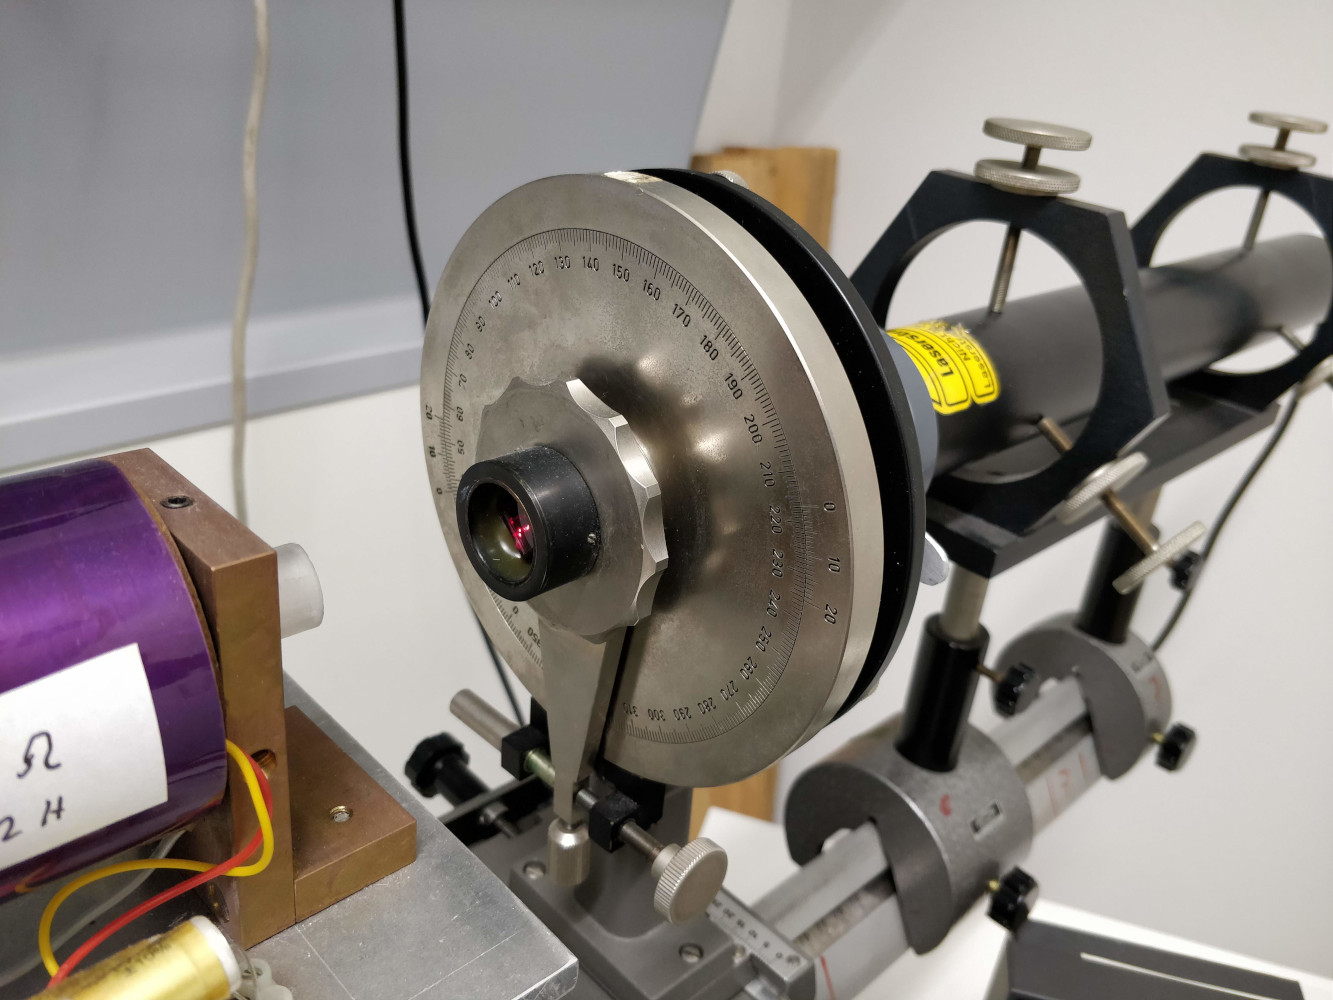
\includegraphics[width=\textwidth]{laser_polariser}
\caption{He-Ne laser and the first polariser}
\label{fig:exp_setup_laser}
\end{subfigure}
\begin{subfigure}[b]{0.45\textwidth}
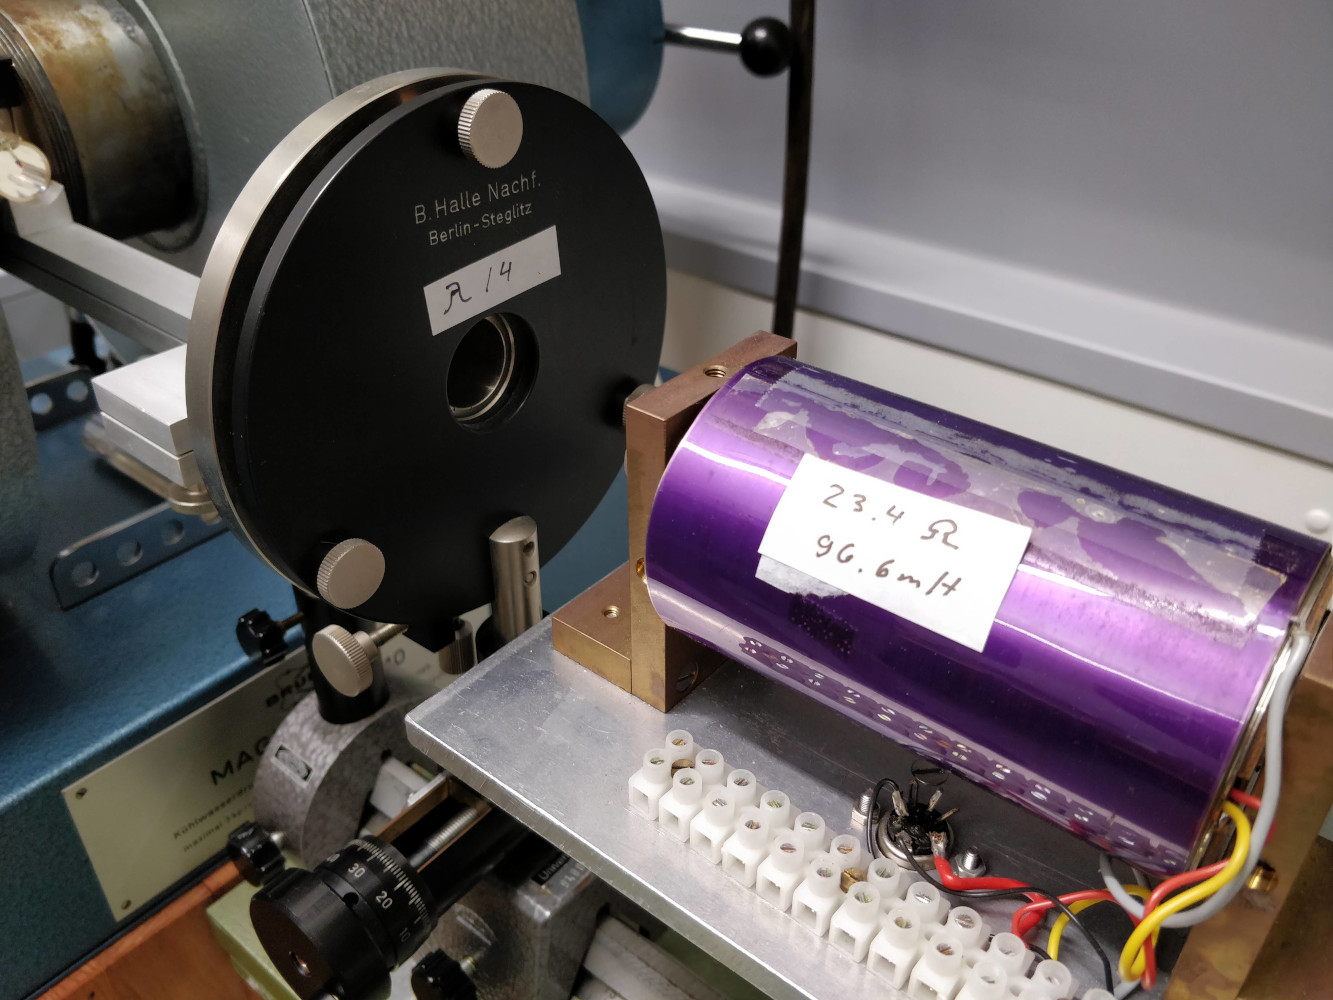
\includegraphics[width=\textwidth]{Faraday_compensator_quarter_plate}
\caption{Faraday compensator and quarter-wave plate}
\label{fig:exp_setup_faraday}
\end{subfigure}\\\vspace{.2cm}
\begin{subfigure}[b]{0.45\textwidth}
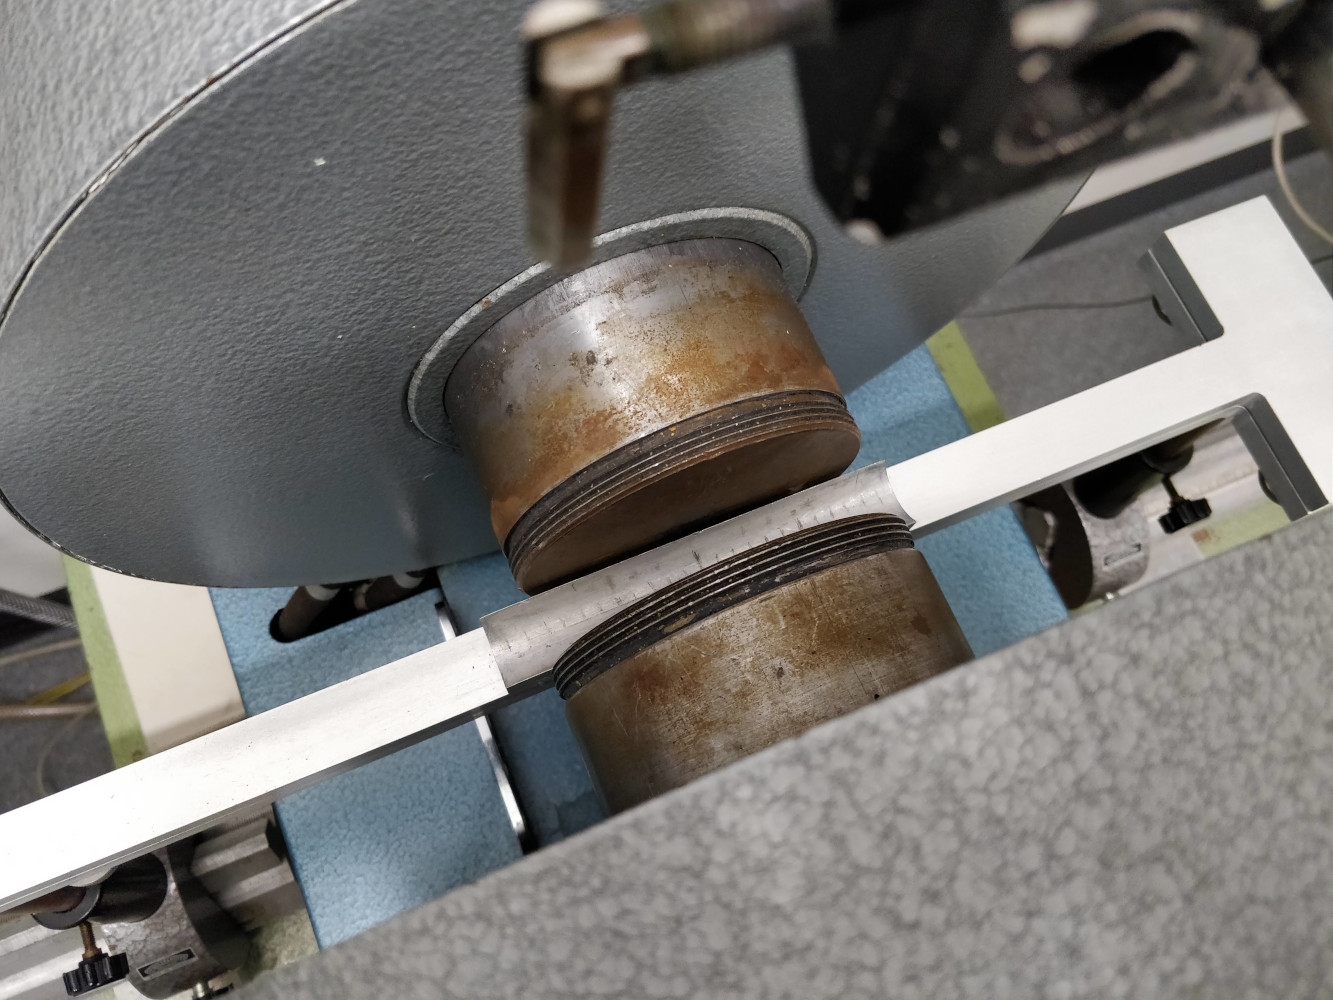
\includegraphics[width=\textwidth]{solenoid}
\caption{Solenoid}
\label{fig:exp_setup_solenoid}
\end{subfigure}
\begin{subfigure}[b]{0.45\textwidth}
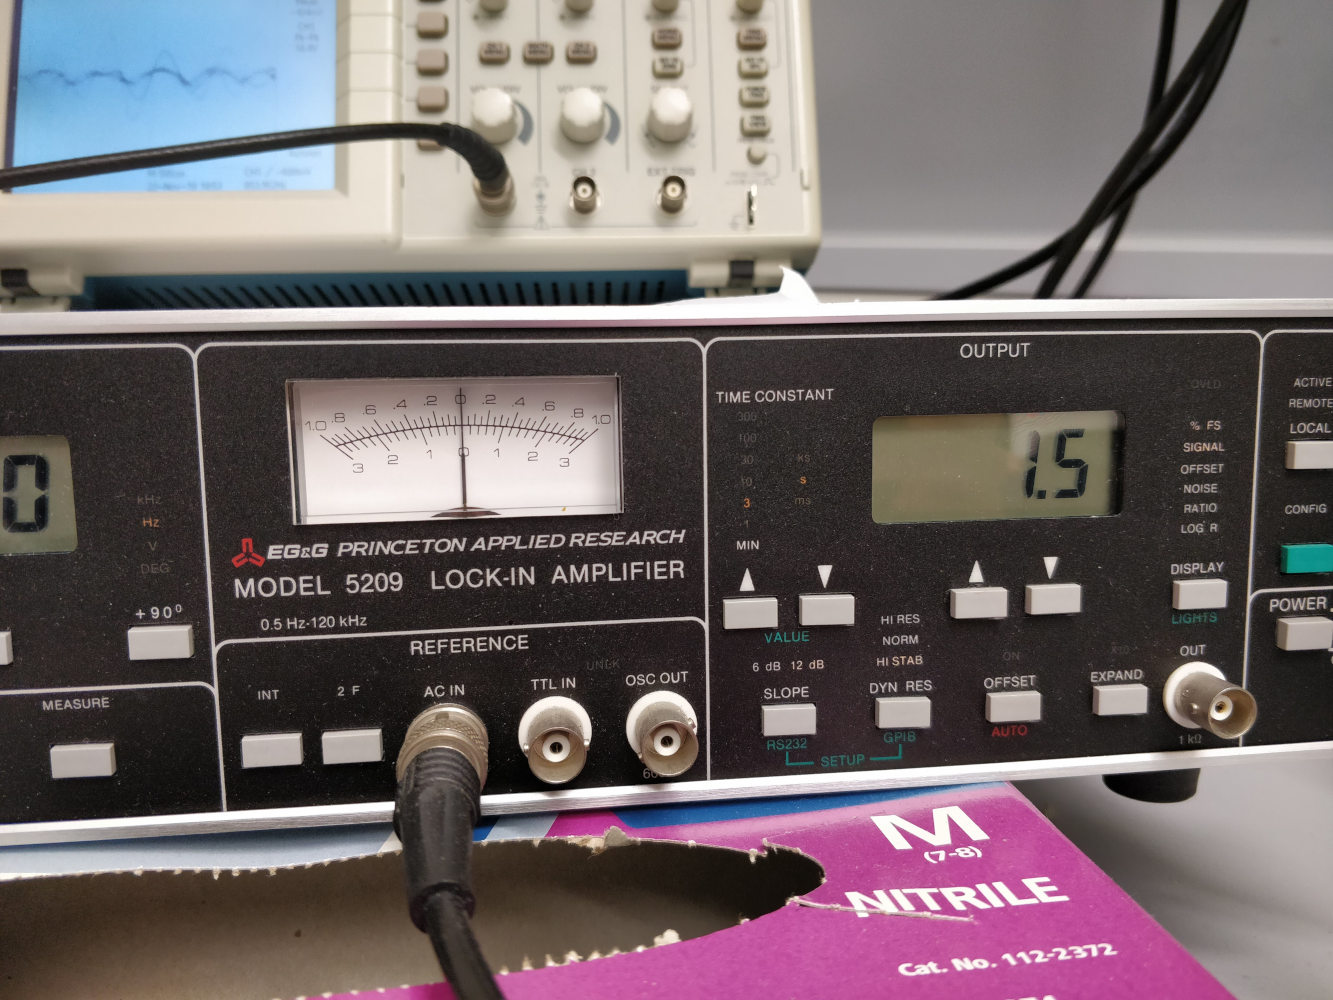
\includegraphics[width=\textwidth]{lock-in}
\caption{Lock-in amplifier}
\label{fig:exp_setup_lockin}
\end{subfigure}
\caption{Some pictures of the experimental setup}\label{fig:exp_setup}
\end{figure}
	
In our experiment, we had the following steps:

\begin{enumerate}
\item The beam of a laser passes through a polariser in order to obtain linear polarization (fig \ref{fig:exp_setup_laser}).
\item By means of Faraday effect (the magnetic field is produced with a solenoid) the direction of the polarization is rotated. This Faraday compensator is shown in (fig \ref{fig:exp_setup_faraday}).
\item A quarter-wave plate set in the same direction of the polarizer produces elliptical polarization if the magnetic effect in the previous step rotates the polarization.
\item We stimulate a birefringence using the Cotton-Mouton effect. The sample is placed in the centre (fig \ref{fig:exp_setup_solenoid}) where the field can be considered (and we will show) constant.
\item The beam passes through an analyser.
\item We measure the intensity of the beam using a photodiode and a lock-in amplifier. In (fig \ref{fig:exp_setup_lockin}) the device is shown for a minimum in intensity.
\end{enumerate}	

Firstly, we minimized the intensity of light skipping step 2. and 4., hence without magnetic fields.  The quarter-wave plate does not provide an elliptical polarization because it has the same direction of the polariser in the first step; setting the analyser we look for the angle that minimizes the gain of the photodiode. After this first step, the angles of the analyser, polariser and quarter-wave plate are left invariant for all the experiment.

Secondly, we insert the sample of step 4. and we apply a magnetic field through it. The Cotton-Mouton effect will produce a retard in the circular polarization. 

Finally, we look for the value of the intensity applied to the solenoid in step 3. that minimizes the gain of the photodiode. 

Let us now calculate the effect of the different optical elements using Jones matrices.

The light produced by the laser after the first polariser can be represented by the Jones vector:

\begin{equation}\label{eq:initial_jones}
J_0=\frac{1}{\sqrt{2}}\left(\frac{1}{1}\right)
\end{equation}

Faraday compensator produces a rotation of the polarisation plane an angle $\theta_F$ given (\ref{verd}) that we can express with the rotation matrix:

\begin{equation}\label{eq:rotation_matrix}
R_F(\theta_F)=
\begin{pmatrix}
\cos\theta_F & -\sin\theta_F \\
\sin\theta_F & \cos\theta_F
\end{pmatrix}
\end{equation}

A quarter-wave plate with its fast axis at an angle $\varphi$ with respect to the horizontal axis produces as phase retardation given by the following Jones Matrix:

\begin{equation}\label{eq:quarter_wave}
W_{\lambda/4}(\varphi)=e^{-i\frac{\pi}{4}}
\begin{pmatrix}
\cos^2\varphi+i\sin^2\varphi & (1-i)\sin\varphi\cos\varphi \\
(1-i)\sin\varphi\cos\varphi & \sin^2\varphi+i\cos^2\varphi
\end{pmatrix}
\end{equation}

Later, we have the sample, that due to the external magnetic field acts as an arbitrary phase retarder given by the following Jones matrix:

\begin{equation}\label{eq:birefringent}
W_{CM}(\theta_{CM})=
\begin{pmatrix}
e^{-i\frac{\delta}{2}} & 0 \\
0 & 1
\end{pmatrix}
\end{equation}

And finally, the analyser which has with its transmission axis perpendicular to the first polariser is given by:

\begin{equation}\label{eq:analyser}
A=\frac{1}{2}
\begin{pmatrix}
\phantom{-}1 & -1 \\
-1 & \phantom{-}1
\end{pmatrix}
\end{equation}

In the first part we set $\theta_F=0$ (i.e. no Faraday magnetic field), $\varphi=\frac{\pi}{4}$ (i.e. the quarter wave plate let the beam unmodified) and $\delta=0$ (i.e. we don't put the sample). In these conditions the final intensity of the beam is zero, we obtain the following equation:

\begin{equation*}
J_f=A\,W_{CM}(0)\,W_{\lambda/4}(\varphi=\pi/4)\,J_0=
\begin{pmatrix}
0\\0
\end{pmatrix}
\end{equation*}
In the same way, when we place the sample and we swich on the magnetic fields, we will set $B_F$ such that the intensity of the light is still zero. In this way we can use the following equality:
\begin{equation*}
J_f=A\,W_{CM}(\delta)\,W_{\lambda/4}(\varphi=\pi/4)\, R_F(\theta_F)\,J_0=
\begin{pmatrix}
0\\0
\end{pmatrix}
\end{equation*}
\begin{equation*}
\Rightarrow\qquad \frac{(1+i)e^{\frac{i\delta}{2}}sin\left( \frac{\delta}{2}-\theta_F\right) }{\sqrt{2}}=0
\end{equation*}
Solving the equation we get $\delta$ as a function of $\theta_F$:
\begin{equation}\label{eq:rel_optical_phase_angle}
\Rightarrow \qquad \delta=2\theta_F
\end{equation}

\section{Materials and methods}\label{mm}
In the first part of the experiment, we measured the magnetic field used to produce the Cotton-Mouton effect in step 4. with a Hall probe. The magnetic field was produced by means of a Helmholtz coil in order to make it as much uniform as possible. According to the Ampère law, the magnetic field can be expressed as:

\begin{equation}
B(I)=\frac{LI}{A}\label{amp}
\end{equation}
where $L$ is the inductance of the coil, $A$ is the surface and $I$ is the current flowing in the coil. In this part, we looked for the region of linearity of the magnetic field in function of the current $I$. The probe was positioned in the middle of the coils; (hence $cos\phi=1$ in \ref{verd}) we took a measurement of the magnetic field by changing the current at steps of \SI{1}{\mA} from \SIrange{-20}{+20}{\mA}. Merging (\ref{verd}) with (\ref{amp}), we get the following formula:
\begin{equation}
\theta_F=\frac{lVL}{A}I\equiv V'I\label{modverd}
\end{equation} where $V'$ is our \emph{modified Verdet constant}.

Secondly, we checked the uniformity of the magnetic field inside the coils in order to position the sample in the region where $\vec{B}$ is uniform.

Thirdly, we verified the linearity of the Faraday effect. The beam of the laser passed respectively through the polarizer, the solenoid of step 2. (the magnetic field had direction parallel to the propagation of light), the analyzer and ended in the photodiode. The solenoid was set in such a way that the magnetic field was parallel to the direction of the laser. Varying the intensity of the current applied to the solenoid we looked for the angle of the analyzer such that the gain of the photodiode was minimized.

The circuit used to produce Faraday effect was composed by a voltage generator, a solenoid and either one or two resistors. Using 2 resistors we will have less current at our disposal. On the contrary, using 1 resistor we will have higher intensities. We took measurements with both the configurations.

Finally, we measured Cotton-Mouton effect. The laser beam in this part used to follow all the steps described in section~\ref{mm}. During this part the magnetic field ($B_{CM}$) applied to one of the three samples was varied from \SIrange{0}{10}{\mA}. For every different $B_{CM}$ we looked for the value of the magnetic field ($B_F$) used to produce Faraday effect (step 2.) such that the gain of the photodiode was minimized.

The laser was a He-Ne laser with $\lambda=\SI{632.8}{\nm}$ and the liquid samples were put in vessels of width $l=\SI{10}{\cm}$.

\newpage

\section{Results and discussion}

\subsection{Characterising magnetic field}

We measured the magnetic field with the probe fixed in the middle for different values of current, first in one direction and then in the other.

\begin{figure}[H]
\centering
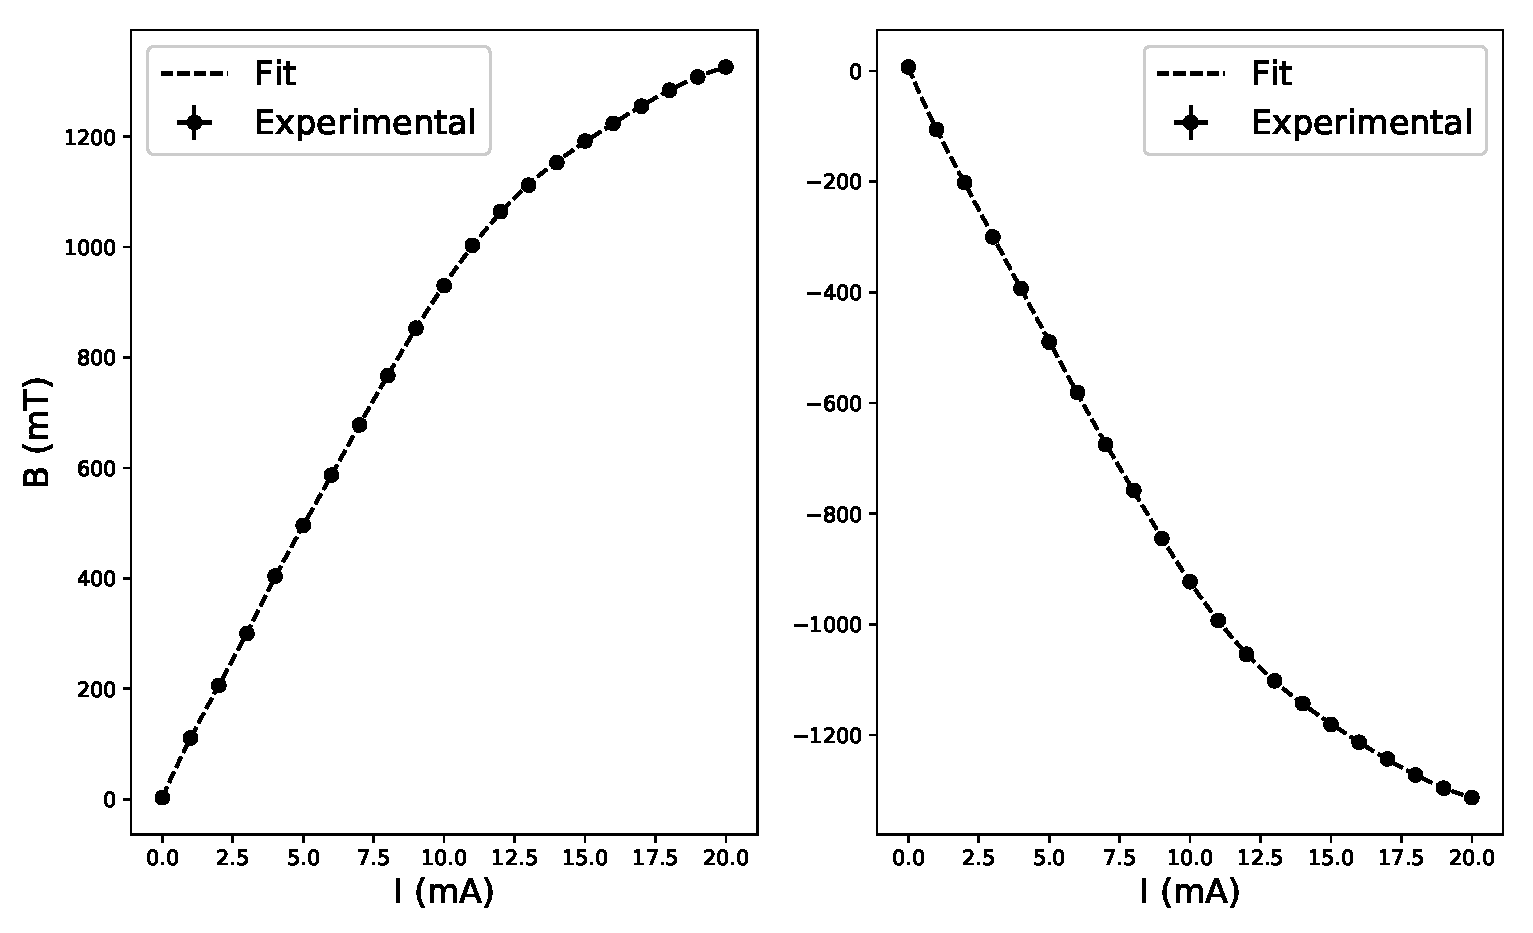
\includegraphics[width=0.9\textwidth]{B_diff_current.eps}
\caption{Magnetic field as a function of current for the two circulating directions with the probe fixed in the middle of the solenoid.}
\label{fig:BvsI}
\end{figure}

Then we measured the magnetic field produced by a fixed current for different positions by moving the probe in steps of \SI{5}{\mm} from one end to the other. First measurement was done for a magnetic field produced by $I=\SI{10}{\mA}$.

\begin{figure}[H]
\centering
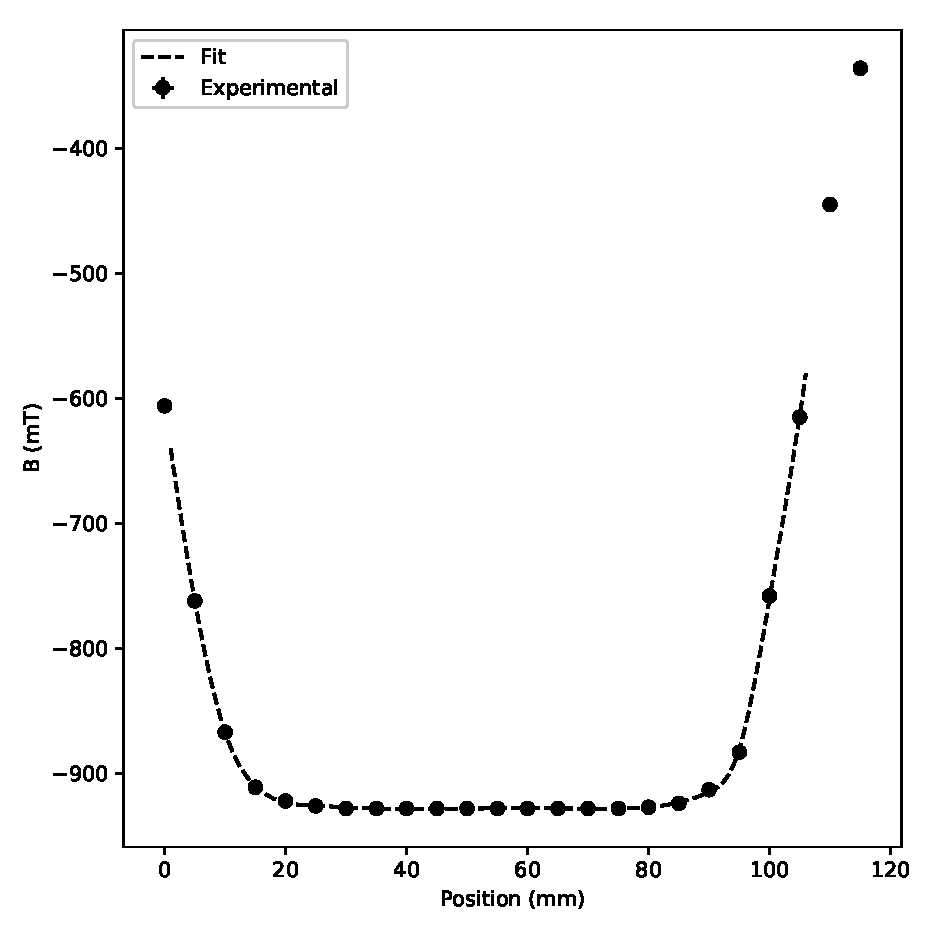
\includegraphics[width=0.55\textwidth]{B_diff_position1.eps}
\caption{Magnetic field as a function of position for a fixed current of \SI{10}{\mA}.}
\label{fig:BvsPos1}
\end{figure}

Two more precise measurements due to a change of scale in the measuring device from \SI{2000}{mT} to \SI{20}{mT} were done later for a fixed value of current of $I=\SI{1}{\mA}$.

\begin{figure}[H]
\centering
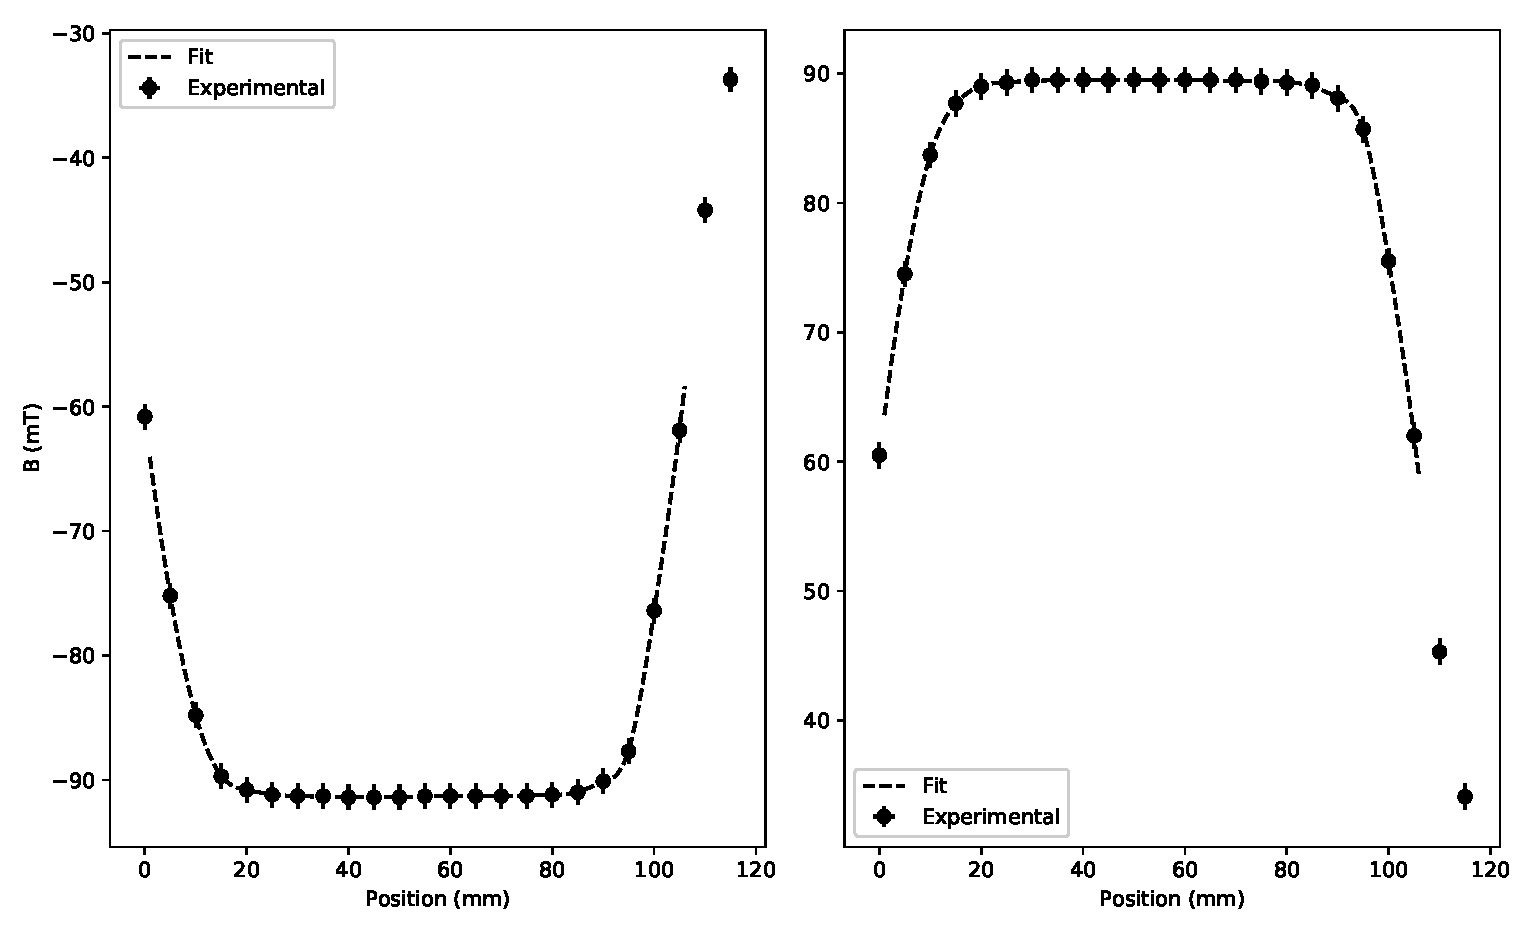
\includegraphics[width=0.9\textwidth]{B_diff_position2.eps}
\caption{Magnetic field as a function of position for a fixed current of \SI{1}{\mA}. Direction of current was changed for each measurement.}
\label{fig:BvsPos2}
\end{figure}

\subsection{Determining modified Verdet constant}

We turned on the laser in order to measure the Faraday effect. For different values of current in the Faraday compensator, i.e. different values of the magnetic field in the direction of the propagation of the light, the angle of the analyser for which we minimised the signal at the detector was recorded. We repeated the measurements for both possible directions of the current and with one and two resistors.

Angles were measured in degrees, minutes and seconds using an optical device. These angles were processed into radians, the offset was subtracted and finally a linear regression was found using the method of least-squares (Figure \ref{fig:FaradayAngle}). The slope is precisely the modified Verdet constant of the Faraday compensator described in (\ref{modverd}), which tells us how much the polarisation plane is rotated by the Faraday effect when applying a current of \SI{1}{mA}.

The following table summarises the values obtained for the Verded constant.

\begin{table}[H]
\centering
\begin{tabular}{ccc}
\toprule
Measurement & $V$ (\si{10^{-5}.\radian/\mA}) & $\delta V$ (\si{10^{-5}.\radian/\mA})\\
\midrule
2 resitors, pos 1 & -3.40 & 0.08 \\
1 resistor, pos 1 & -3.47 & 0.04 \\
2 resistors, pos 2 & -3.39 & 0.03 \\
1 resistors, pos 2 & -3.4 & 0.1 \\
\bottomrule
\end{tabular}
\caption{Values obtained for the modified Verdet constant with one and two resistors and for both directions of the current in the Faraday compensator.}
\label{table:verdet}
\end{table}

Uncertainties $\delta V$ were calculated by computing the square root of the covariances obtained from the least-squares fit.

For computing the Cotton-Mouton constants in the following section, we use the modified Verdet constant obtained using two resistors and the current circulating in the second position.

\begin{equation}\label{val:verdet}
V'=\SI{-3.39\pm0.03}{\num{e-5}.\radian/\mA}
\end{equation}

\begin{figure}[H]
\centering
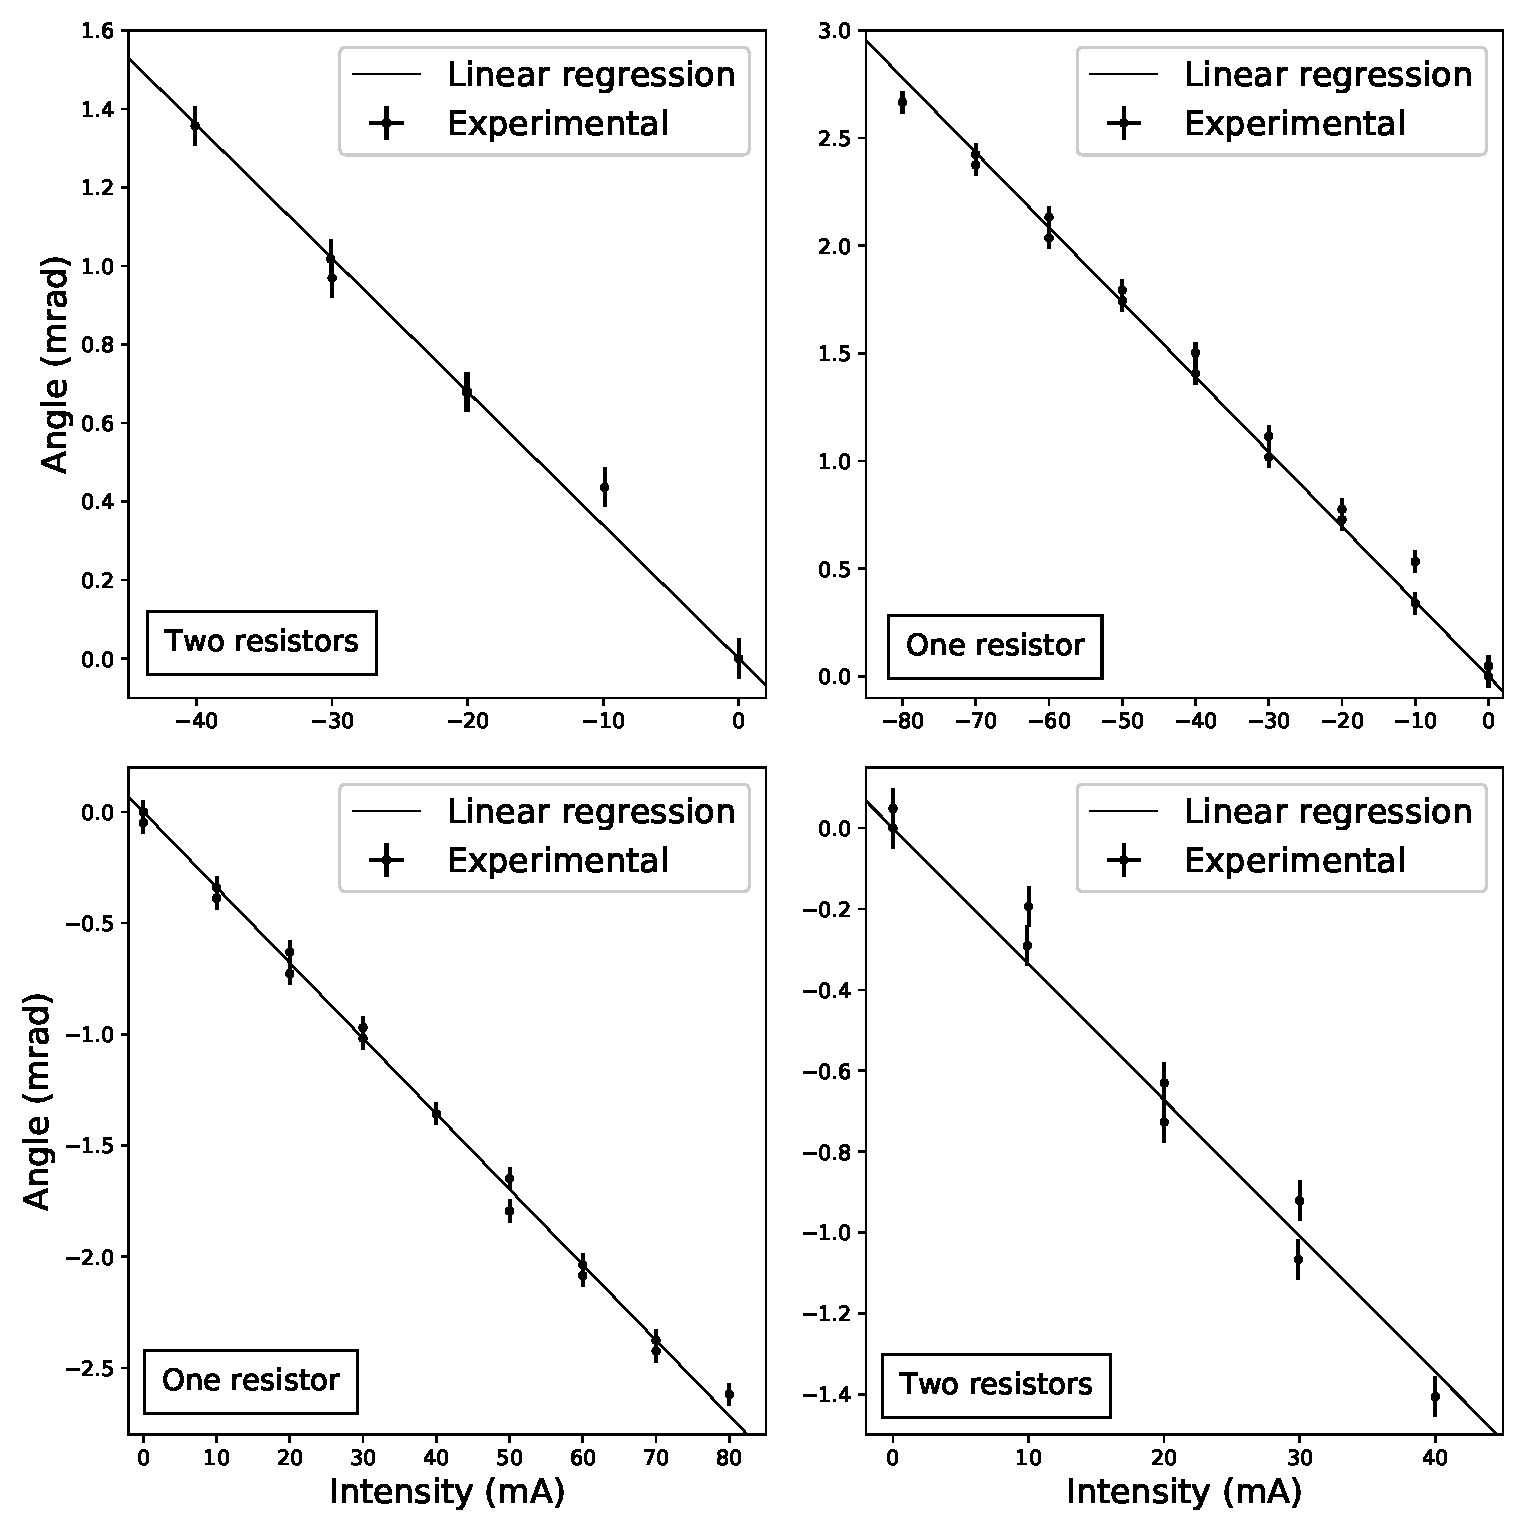
\includegraphics[width=\textwidth]{Angle_diff_intensity2.eps}
\caption{Magnetic field as a function of position for a fixed current of \SI{1}{\mA}. Direction of current was changed for each measurement.}
\label{fig:FaradayAngle}
\end{figure}

\subsection{Measuring Cotton-Mouton effect}

We measured the Cotton-Mouton effect by finding the rotation in the polarisation plane of the light (using the Faraday compensator) which minimised the intensity at the analyser. As explained before, the Cotton-Mouton effect produces an optical retardation, an optical phase given by equation (\ref{eq:CME}) that makes our polarisation of the light no longer aligned with the quarter-wave plate. The result is an elliptical polarisation, whose different components will travel at different speeds in the birefringent material.

Experimentally, we measured the current intensity in the Faraday compensator at which we found the minimum for different values of current in the solenoid, in steps of \SI{2}{\mA} both increasing the current and decreasing it. When we got to the maximum possible current in the solenoid for which we were able to compensate using the Faraday effect, we reduce the current \SI{1}{\mA} and then again in steps of \SI{2}{\mA}, so we obtained measurements for every \si{\mA}. Experimental data is shown in Appendix \ref{app:experimental_data}.

The Cotton-Mouton constants for the three samples can be obtained by plotting $\Delta n$ against the square of the magnetic field applied to the sample, and doing a linear regression to find the slope, which will be $C\lambda$ as shown in (\ref{eq:Delta_n}). $\Delta n$ can be obtained from the measured current in the Faraday compensator using (\ref{eq:optical_phase}) and (\ref{eq:rel_optical_phase_angle}), and the square of the magnetic field from the current measured in the solenoid and the interpolation done in (fig \ref{fig:BvsI}) during the characterising of the field.

Explicitly, we get the following equation for $\Delta n$ as a function of the measured $I_F$:

\begin{equation}\label{eq:delta_n}
\Delta n(I_F)=\frac{1}{\pi}\frac{\lambda}{L}V'I_F\;,
\end{equation}
where $V'$ is the modified Verdet constant determined in (\ref{val:verdet}) and $\lambda$ and $L$ are known.

The uncertainty of this value is computed using propagation of errors and we get:

\begin{equation}\label{eq:d_delta_n}
\delta\Delta n=\left|\frac{\partial\Delta n}{\partial V'}\right|\delta V'+\left|\frac{\Delta n}{\partial I_F}\right|\delta I_F=\frac{1}{\pi}\frac{\lambda}{L}\big(I_F\delta V'+V'\delta I_F\big)
\end{equation}

In the following table, the CM constants obtained for the three samples are presented:

\begin{table}[H]
\centering
\begin{tabular}{ccc}
\toprule
Sample & $C$ (\si{10^{-3}.\tesla^{-2}.\m^{-1}}) & $\delta C$ (\si{10^{-3}.\tesla^{-2}.\m^{-1}})\\
\midrule
Toluene & 3.5 & 0.5 \\
Mesitylene & 4.54 & 0.06 \\
Carbon disulfide & 3.48 & 0.04 \\
\bottomrule
\end{tabular}
\caption{Values obtained experimentally for the Cotton-Mouton constant for the three samples: Toluene (C$_7$H$_8$), Mesitylene (C$_9$H$_{12}$) and Carbon disulfide (CS$_2$).}
\label{table:CM}
\end{table}


\begin{figure}[H]
\centering
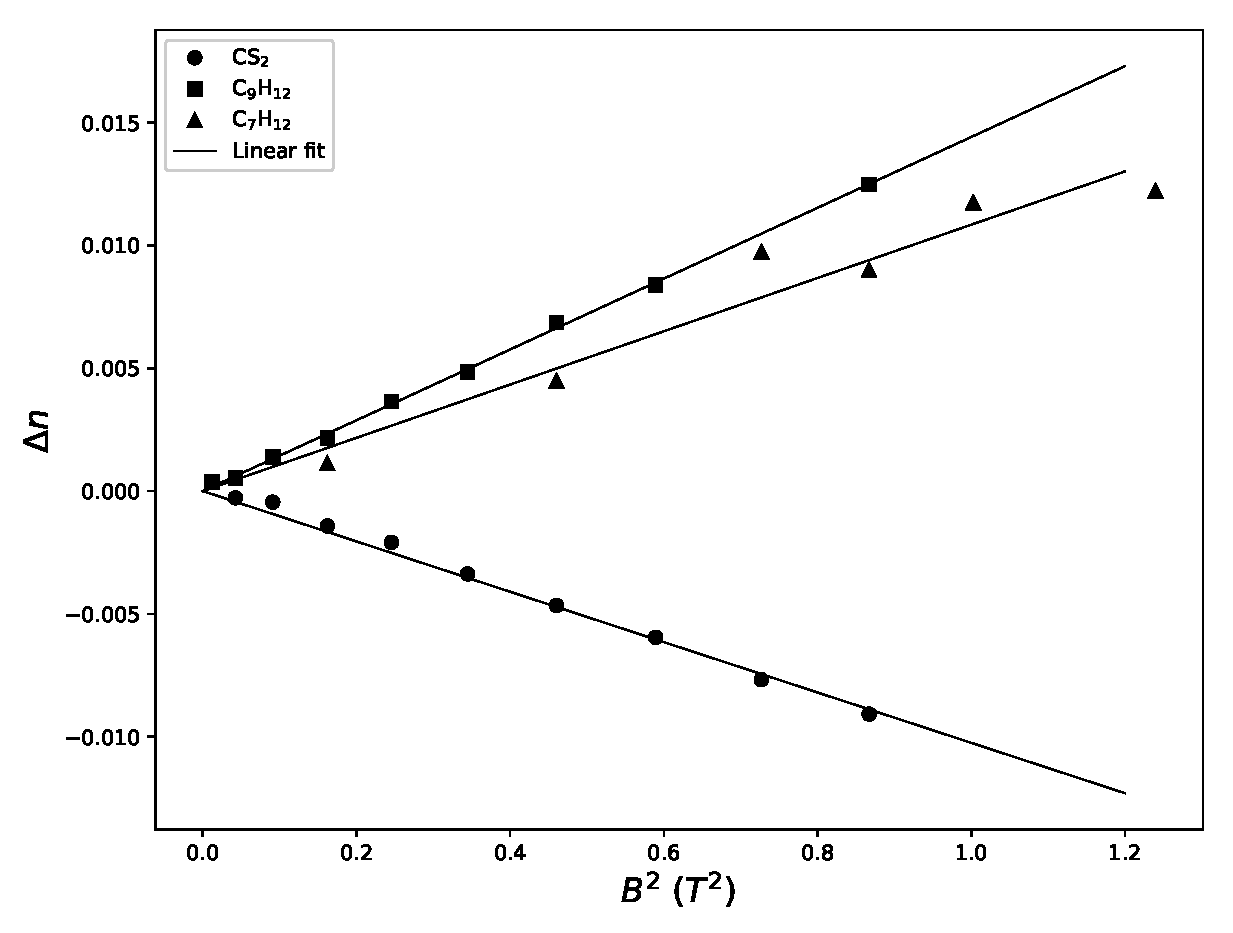
\includegraphics[width=0.9\textwidth]{CM_consts.eps}
\caption{$\Delta n$ plotted against the square of the magnetic field applied to the sample. $\Delta n$ is obtained from the measured current in the Faraday compensator using eqs.~\eqref{eq:optical_phase} and \eqref{eq:rel_optical_phase_angle}. $B^2$ is obtained interpolating (see Figure \ref{fig:BvsI}) from the measured current in the solenoid. The negative slope for the Carbon disulfide is due to the fact that we change the direction of the current (as shown in Appendix \ref{app:experimental_data}). It was not modified to avoid overlapping with experimental points from Toluene. From eq.~\eqref{eq:Delta_n} we can see that the slope is proportional to the Cotton-Mouton constant. Experimental obtained values are shown in Table \ref{table:CM}.}
\label{fig:CM_const}
\end{figure}


\section{Conclusions}
As expected, the Cotton-Mouton constant is negative for the carbon disulfide and positive for the other samples. This fact is clearly shown in Figure \ref{fig:CM_const}, where the fit of CS$_2$ has a negative slope.

Toluene sample was the most difficult sample to measure because it is the less active sample and also due to some variance in the signal generator for the lock-in amplifier during the measurement, which led to a measurement an order of magnitude worse than the other two samples by checking $\delta C/C$.

\vfill
{\color{white}\cite{wilson1997simple}\cite{note19923}\cite{montarou2004two}\cite{freiser1968survey}}
\bibliographystyle{unsrt}
\bibliography{references}

\newpage
\begin{appendices}
\section{Experimental data}\label{app:experimental_data}

\begin{figure}[H]
\centering
\begin{subfigure}[b]{0.55\textwidth}
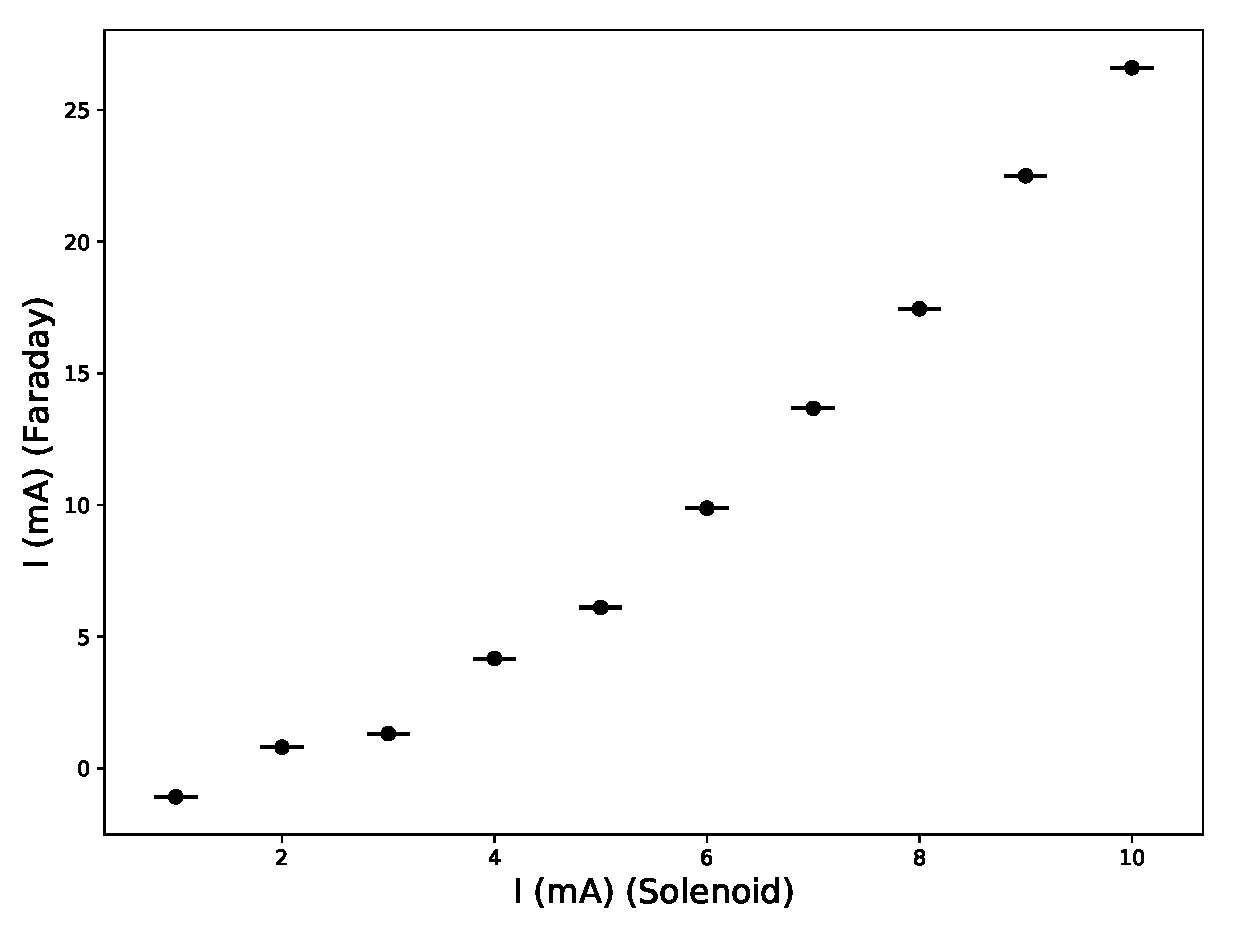
\includegraphics[width=\textwidth]{sample3}
\caption{Carbon disulfide (CS$_2$)}
\label{fig:CME_sample3}
\end{subfigure}\\\vspace{.2cm}
\begin{subfigure}[b]{0.55\textwidth}
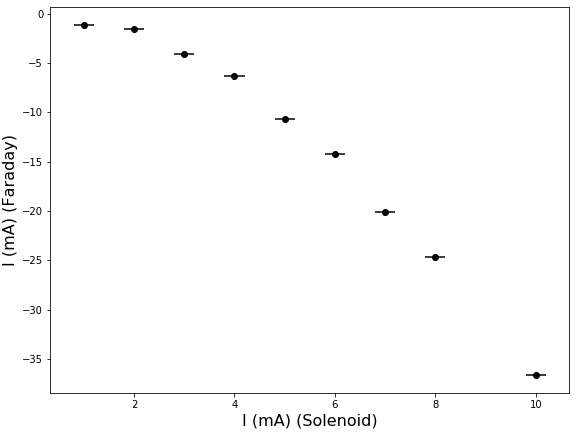
\includegraphics[width=\textwidth]{sample2}
\caption{Mesitylene (C$_9$H$_{12}$)}
\label{fig:CME_sample2}
\end{subfigure}\\\vspace{.2cm}
\begin{subfigure}[b]{0.55\textwidth}
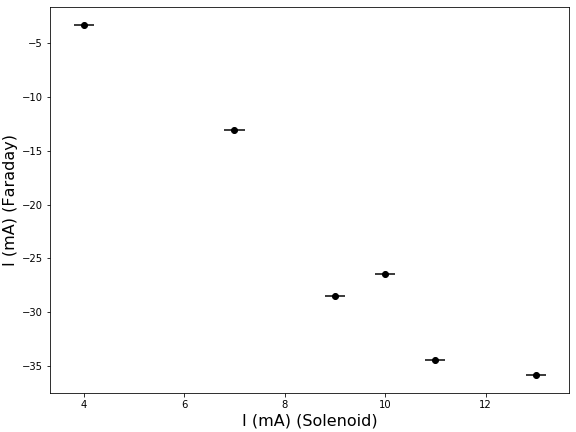
\includegraphics[width=\textwidth]{sample1}
\caption{Toluene (C$_7$H$_8$)}
\label{fig:CME_sample1}
\end{subfigure}
\caption{CME measured for three different samples. Current intensity of the Faraday compensator is plotted against the current in the solenoid where the sample is placed.}
\label{fig:CME}
\end{figure}

\end{appendices}

\end{document}